\begin{definition}
	Eine Folge $(X_n)_{n \in \N_0}$ von reellen Zufallsvariablen auf $(\O,\F\,\P)$ heißt \begriff{Martingal}, falls
	\begin{enumerate}
		\item $\E[\abs{X_n}] < \infty$ also $X_n \in \Ln{1}(\P)\forall n \in \N_0$
		\item $\E[X_{n-1} \mid X_0, X_1, \dots, X_n] = X_0, \P\text{-f.s. }\forall n \in \N$
	\end{enumerate}
	Die Folge $(X_n)_{n\in \N}$ heißt \begriff{Super-/Submartingal}, falls 1. und folgendes gilt
	\begin{enumerate}
		\item $\E[X_{n-1} \mid X_0, X_1, \dots, X_n] \le /\ge X_0, \P\text{-f.s. }\forall n \in \N$
	\end{enumerate} 
\end{definition}
\begin{example}
	Sei $(Y_n)_{n\in \N}$ Folge von u.i.v. Zufallsvariablen auf $(\O,\F,\P)$ in $\Ln{1}(\P)$, reellwertig mit $\E[Y_1] = 0$. Dann ist $(X_n)_{n\in \N}$ mit 
	\begin{align*}
		X_0 = 0 \und X_n = \sum_{k=1}^n Y_k \quad n \ge 1
	\end{align*}
	ein Martingal, denn
	\begin{enumerate}
		\item $\E[\abs{X_n}] \le \sum_{k=1}^n \E[\abs{Y_k}] < \infty$
		\item 
		\begin{align*}
			\E[X_{n+1}\mid X_0, \dots, X_n] &= \E[X_n + Y_{n+1} \mid X_0 , ... , X_n] = \E[X_n \mid X_0, ... X_n] + \E[Y_{n+1} \mid X_0, ... X_n]\\
			&= X_n + \E[Y_{n+1}] = X_n \quad \P\text{-f.s. } \forall n \in \N
		\end{align*}
		Für $\E[Y_1] \ge / \le 0$ erhält man dementsprechend ein Sub-/Supermartingal.
	\end{enumerate}
\end{example}
%Hier ist die letzte Vorlesung noch fehlend, wird vielleicht nach der Prüfung ergänzt, mal schaun ... ;)
\begin{example}
	\proplbl{11_3}
	Sei $(X_n)_{n\in \N}$ ein (Super-/Sub-)Martingal auf $(\O,\F,\P)$ und $(C_n)_{n\in \N}$ eine Folge von beschränkten Zufallsvariablen in $[0,\infty)$, sodass $C_n$ $\sigma(X_0,\dots,X_{n-1})$-messbar ist. Dann ist $(Y_n)_{n\in \N_0}$ mit
	\begin{align*}
		Y_0 := 0 \quad Y_n = \sum_{i=1}^n C_i (X_i -X_{i-1}) \quad \text{ für }n \le 1
	\end{align*}
	ein (Super-/Sub-)Martingal ($\nearrow$ Übung).\\ %TODO maybe format better?
	\ul{Interpretation:}\\
	\begin{itemize}
		\item $(X_i - X_{i-1})$ entspricht Gewinn in Runde $i$ pro Einsatzeinheit ($X$ Martingal $\rightsquigarrow$ faires Spiel mit Supermartingal $\rightsquigarrow$ nachteilig und Submartingal $\rightsquigarrow$ vorteilig)
		\item $C_i$ entspricht Einsatz in Runde $i$
		\item $Y_n$ entspricht Gewinn nach $n$ Runden
	\end{itemize}
\end{example}
\begin{lemma}[\person{Doob}'s Upcrossing Lemma]
	Sei $(X_n)_{n\in \N_0}$ ein Supermartingal auf $(\O,\F,\P)$ und für $a,b \in \R,N\in \N$. Sei $U_N[a,b] = \#$ Upcrossings von $[a,b]$ durch $X$ bis zur Zeit $N$:
	\begin{center}
		\tikzset{every picture/.style={line width=0.75pt}} %set default line width to 0.75pt        
		
		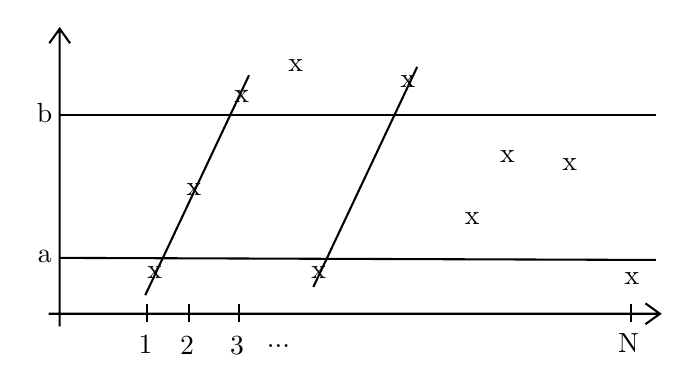
\begin{tikzpicture}[x=0.75pt,y=0.75pt,yscale=-1,xscale=1]
		%uncomment if require: \path (0,300); %set diagram left start at 0, and has height of 300
		
		%Shape: Axis 2D [id:dp16446481605444763] 
		\draw  (7.94,186.76) -- (302.5,186.76)(13.28,49.42) -- (13.28,192.83) (295.5,181.76) -- (302.5,186.76) -- (295.5,191.76) (8.28,56.42) -- (13.28,49.42) -- (18.28,56.42)  ;
		%Straight Lines [id:da28338828151955764] 
		\draw    (13.5,159.83) -- (300.5,160.83) ;
		
		
		%Straight Lines [id:da8271221523951781] 
		\draw [color={rgb, 255:red, 0; green, 0; blue, 0 }  ,draw opacity=1 ]   (13.5,90.83) -- (300.5,90.83) ;
		
		
		%Straight Lines [id:da6380294556294152] 
		\draw    (104.5,71.83) -- (54.5,177.83) ;
		
		
		%Straight Lines [id:da9952421299305323] 
		\draw    (185.5,67.83) -- (135.5,173.83) ;
		
		
		%Straight Lines [id:da9651863477189166] 
		\draw    (55.5,181.83) -- (55.5,190.83) ;
		
		
		%Straight Lines [id:da018191406991399095] 
		\draw    (75.5,181.83) -- (75.5,190.83) ;
		
		
		%Straight Lines [id:da2253324698452538] 
		\draw    (99.5,181.83) -- (99.5,190.83) ;
		
		
		%Straight Lines [id:da32014991281507543] 
		\draw    (288.5,181.83) -- (288.5,190.83) ;
		
		
		
		% Text Node
		\draw (6,159) node  [align=left] {a};
		% Text Node
		\draw (6,90) node  [align=left] {b};
		% Text Node
		\draw (59,167) node  [align=left] {x};
		% Text Node
		\draw (78,127) node  [align=left] {x};
		% Text Node
		\draw (101,82) node  [align=left] {x};
		% Text Node
		\draw (138,167) node  [align=left] {x};
		% Text Node
		\draw (127,67) node  [align=left] {x};
		% Text Node
		\draw (181,75) node  [align=left] {x};
		% Text Node
		\draw (212,141) node  [align=left] {x};
		% Text Node
		\draw (259,115) node  [align=left] {x};
		% Text Node
		\draw (229,111) node  [align=left] {x};
		% Text Node
		\draw (289,170) node  [align=left] {x};
		% Text Node
		\draw (54.67,201.42) node  [align=left] {1};
		% Text Node
		\draw (74.67,202.08) node  [align=left] {2};
		% Text Node
		\draw (98.67,202.08) node  [align=left] {3};
		% Text Node
		\draw (287.33,200.75) node  [align=left] {N};
		% Text Node
		\draw (118.67,202.08) node  [align=left] {...};
		
		\end{tikzpicture}
	\end{center}
	d.h.
	\begin{align*}
		U_N[a,b](\omega) = \{\max k\in \N_0&\colon \exists 0 \le S_1 < t_1 < S_2 <t_2 < ... < s_k < t_k \le N \\
		&\colon X_{s_i} < a, X_{t_i}>b, i \in \set{1,...,k}\}
	\end{align*}
	Dann gilt
	\begin{align*}
		\E[U_N[a,b]] \le \frac{\E[(X_N - a)^-]}{b-a}
	\end{align*}
\end{lemma}
\begin{proof}
	Interpretiere $(X_i - X_{i-1})$ als Gewinn in Spielrunde $i$ pro Einsatzeinheit. Wähle als Spielstrategie
	\begin{align*}
		C_1 &:= \indi_{\set{X_0 < a}}\\
		C_n &:= \indi_{\set{C_{n-1} =1}}\indi_{\set{X_{n-1} \le b}} + \indi_{\set{C_{n-1} =0}}\indi_{\set{X_{n-1} \le a}}
	\end{align*}
	Dann ist $(C_n)_{n\in \N}$ beschränkt, nicht-negativ und $C_n$ ist $\sigma(X_0,\dots,X_{n-1})$ messbar. Nach \cref{11_3} ist $(Y_n)_{n\in \N_0}$ mit
	\begin{align*}
		Y_0 &= 0\\
		Y_n &= \sum_{i=1}^n C_i (X_i - X_{i-1})
		\intertext{ein Superimartingal. Es folgt}
		\E[Y_n] &= \E[\E[Y_N \mid Y_0,...,Y_{N-1}]] \le \E[Y_{N-1}] \le \dots \le \E[Y_0] = 0
		\intertext{Zudem gilt $\forall \omega \in \O$}
		Y_N(\omega) &\ge (b-a)U_N[a,b] - (X_N(\omega)-a)^-\\
		\implies (b-a)\E[U_N[a,b]] &\le \E[Y_N] + \E[(X_N - a)^-]\\
		&\le \E[(X_N -a)^-] %TODO big or small ``n''?
	\end{align*}
\end{proof}
\begin{proposition}[CLT für Martingale]
	Sei $(X_n)_{n\in \N_0}$ ein Martingal mit $X_n \in \Ln{2}(\P)\forall n \in \N_0$, so dass $X_0 = 0$ und 
	\begin{align*}
		\E[\Delta^2_n \mid \F_{n-1}] = \sigma^2
	\end{align*}
	deterministisch ist, wobei
	\begin{align*}
		\Delta_n := X_n - X_{n-1} \und \F_n := \sigma(X_0,\dots, X_n)
	\end{align*}
	Gilt zudem die \person{Lindberg}- Bedingung für Martingale
	\begin{align*} %TODO fix alignment please
		\forall \epsilon > 0 \colon \lim_{n\to \infty} 1/s_n^2 \sum_{k=1}^n \E[\Delta_k^2 \indi_{\abs{\Delta_k}> \epsilon s_n}\mid \F_{k-1}] = 0
		\intertext{mit $s_n^2 = \sum_{k=1}^n \sigma_k^2$. Dann folgt}
		\frac{x_n}{s_n} \xrightarrow[\d]{n \to \N} Z \sim \normal(0,1)
	\end{align*}
	Die Folge $(\F_n)_{n\in \N}$ ist eine ``Filtration''.
\end{proposition}
\begin{proof}
	Ähnlich zum Beweis des CLT nach \person{Lindberg}-\person{Feller}:
	\begin{align*}
		\E[e^{\ii u \Delta_k}\mid \F_{k-1}] = 1+ 
	\end{align*}
\end{proof}